\chapter{Wavelet Transformation} \lhead{\emph{Wavelet Transformation}}


This chapter provides a comprehensive overview of both the continuous and discrete wavelet transforms. Firstly, I will define Wavelets and 
showcase the mathematical theory behind the continuous wavelet transform (CWT). From there I will cover the discrete wavelet transform (DWT) 
and the fast wavelet transform, which allows for efficient computation of the DWT. With all that mathematical machinery in place I will then 
discuss how to use the wavelet transformation for noise estimation and denoising in a simple and effective manner.

I will note here that definitions and notations of wavelet theory are not consistent across literature. 
This issue is compiled by the fact that authors also use different definitions for the Fourier transform 
(i.e. different placing of the normalization factor), which underlies much of the wavelet theory. I followed \cite{sauer-notes},
\cite{mallat2008wavelet} and \cite{shah2022wavelet} for the definitions and theorems presented in this chapter but I did have to adapt them in part to be consistent. 

\section{Continuous Wavelet Transformation}
The fundamental idea behind the wavelet transformation is to analyze through the scale. Wavelets are used in the wavelet transformation the same way sin and cos are used
in the Fourier transformation. In the Fourier transformation, a function is transformed to a new basis given by sin and cos functions in frequency space.
Note that the sin and cos functions do not appear in the definition of FT introduced earlier because we only used the $e^{ikx}$. These functions 
are connected with the identity $e^{ikx} = cos(kx) + i \sin(kx)$.

The basis functions of the Fourier transform are localized in the frequency domain, each sin/cos has a single frequency, but not in the time domain,
where they are periodic and non-vanishing. This means that for periodic,
continuous signals the Fourier transform only needs a small amount of coefficients to obtain a good approximation of the signal.
In addition, noise limited to certain frequencies can be easily detected and filtered. 

Local signals containing discontinuities, on the other hand, cannot be approximated easily and one needs a large amount of Fourier coefficients to approximate them well.
Furthermore, localized time information is stored in the phase of the Fourier transformation, so modifications to the signals in frequency space
e.g. filtering may corrupt transient time information, leading to unwanted side effects.

These problems are addressed by wavelet transformations. Wavelets are, just like sin and cos in the Fourier transformation, used as basis functions
to represent a signal in the frequency domain. The major difference is that wavelets are localized in time and frequency domain. 
Therefore, wavelets are well-suited to approximate data containing sharp discontinuities. 
Another advantage of wavelets is that their width in time and frequency can vary.
This way one has long low frequency basis functions for frequency analysis and short basis functions to isolate discontinuities. The idea is illustrated
in figure \ref{fig:wavelet_trafo_sketch}.

\begin{figure}
    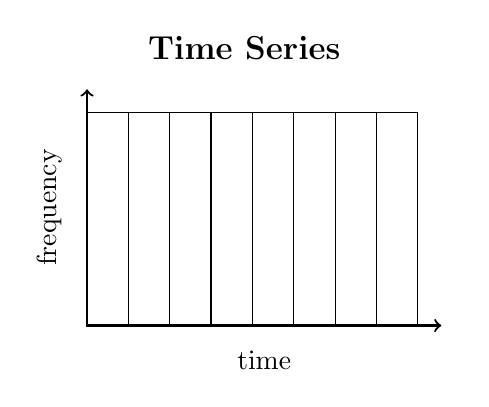
\begin{tikzpicture}[scale=1.5]
        % Draw axes
        \draw [<->,thick] (0,2) node (yaxis) [above] {}
            |- (3,0) node (xaxis) [right] {};

        \node[below=0.2cm] at (1.5, 0) {time};
        \node[rotate=90,above=0.2cm] at (0, 1) {frequency};
        \draw (2.8,0) coordinate (e_1) -- (2.8,1.8) coordinate (e_2);
        \draw (0,1.8) coordinate (e_3) -- (2.8,1.8) coordinate (e_2);

        \foreach \x in {0,...,8}
           {
                \draw (0.35*\x, 0) coordinate (vs_\x) -- (0.35*\x, 1.8) coordinate (ve_\x);
           }

        \node[above,font=\large\bfseries] at (current bounding box.north) {Time Series};
    \end{tikzpicture}%
\qquad
    \hspace{1cm}
    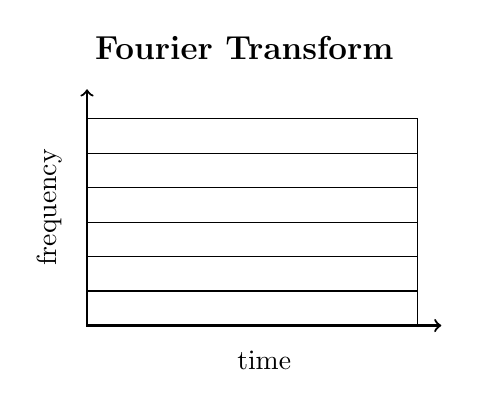
\begin{tikzpicture}[scale=1.5]
        % Draw axes
        \draw [<->,thick] (0,2) node (yaxis) [above] {}
            |- (3,0) node (xaxis) [right] {};

        \node[below=0.2cm] at (1.5, 0) {time};
        \node[rotate=90,above=0.2cm] at (0, 1) {frequency};
        \draw (2.8,0) coordinate (e_1) -- (2.8,1.75) coordinate (e_2);

        \foreach \y in {0,...,6}
           {
                \draw (0, 0.292*\y) coordinate (hs_\y) -- (2.8, 0.292*\y) coordinate (he_\y);
           }
            
        \node[above,font=\large\bfseries] at (current bounding box.north) {Fourier Transform};
    \end{tikzpicture}

    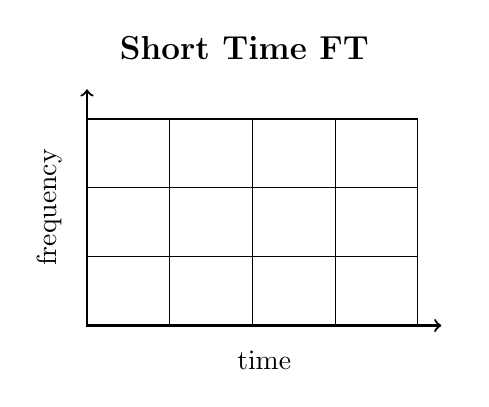
\begin{tikzpicture}[scale=1.5]
        % Draw axes
        \draw [<->,thick] (0,2) node (yaxis) [above] {}
            |- (3,0) node (xaxis) [right] {};

        \node[below=0.2cm] at (1.5, 0) {time};
        \node[rotate=90,above=0.2cm] at (0, 1) {frequency};
        \draw (2.8,0) coordinate (e_1) -- (2.8,1.75) coordinate (e_2);

        \foreach \y in {0,...,3}
           {
                \draw (0, 0.583*\y) coordinate (hs_\y) -- (2.8, 0.583*\y) coordinate (he_\y);
           }

           \foreach \x in {0,...,4}
           {
                \draw (0.7*\x, 0) coordinate (vs_\x) -- (0.7*\x, 1.75) coordinate (ve_\x);
           }
            
        \node[above,font=\large\bfseries] at (current bounding box.north) {Short Time FT};
    \end{tikzpicture}
    \qquad
    \hspace{1cm}
    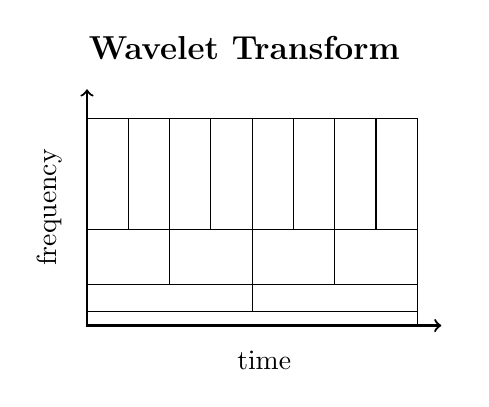
\begin{tikzpicture}[scale=1.5]
        % Draw axes
        \draw [<->,thick] (0,2) node (yaxis) [above] {}
            |- (3,0) node (xaxis) [right] {};

        \node[below=0.2cm] at (1.5, 0) {time};
        \node[rotate=90,above=0.2cm] at (0, 1) {frequency};
        \draw (2.8,0) coordinate (e_1) -- (2.8,1.75) coordinate (e_2);

        %horizontal lines
        \draw (0, 0.33*0.35) coordinate (hs_1) -- (2.8, 0.33*0.35) coordinate (he_1);
        \draw (0, 0.35) coordinate (hs_2) -- (2.8, 0.35) coordinate (he_2);
        \draw (0, 2.33*0.35) coordinate (hs_3) -- (2.8, 2.33*0.35) coordinate (he_3);
        \draw (0, 5*0.35) coordinate (hs_4) -- (2.8, 5*0.35) coordinate (he_4);

        %vertical lines
        \draw (0.466*3, 0.33*0.35) coordinate (vs_1) -- (0.466*3, 1.75) coordinate (ve_1);

        \draw (0.466*1.5, 0.35) coordinate (vs_21) -- (0.466*1.5, 1.75) coordinate (ve_21);
        \draw (0.466*4.5, 0.35) coordinate (vs_22) -- (0.466*4.5, 1.75) coordinate (ve_22);

        \draw (0.466*0.75, 2.33*0.35) coordinate (vs_31) -- (0.466*0.75, 1.75) coordinate (ve_31);
        \draw (0.466*2.25, 2.33*0.35) coordinate (vs_32) -- (0.466*2.25, 1.75) coordinate (ve_32);
        \draw (0.466*3.75, 2.33*0.35) coordinate (vs_33) -- (0.466*3.75, 1.75) coordinate (ve_33);
        \draw (0.466*5.25, 2.33*0.35) coordinate (vs_34) -- (0.466*5.25, 1.75) coordinate (ve_34);

        \node[above,font=\large\bfseries] at (current bounding box.north) {Wavelet Transform};
    \end{tikzpicture}
    \caption[Schematic overview of time/frequency resolution of different transformations]{A schematic overview of the time and 
    frequency resolutions of the different transformations in comparison with the original time-series dataset. 
    The size and orientation of the blocks indicate how small the features are that we can distinguish in the time and frequency domain.}
    \label{fig:wavelet_trafo_sketch}
\end{figure}

For a more mathematically precise formulation, let us first define a Wavelet

\begin{definition}[Wavelet]
    A function $\psi \in L^{2}(\mathbb{R})$ is called a Wavelet if it satisfies the following conditions

    \begin{enumerate}
        \item mean free $\int_{\mathbb{R}} \psi (t) dt = 0$
        \item normalized $\|\psi \|_2 = \sqrt{\int_{\mathbb{R}} \psi(t) \psi^{\ast}(t) dt} = 1$
        \end{enumerate}%
        In many cases an additional condition is required:
        \begin{enumerate}[resume*]
        \item admissibility $\int_{\mathbb{R}} \frac{\hat{\psi}(\omega) \hat{\psi}^{\ast}(\omega)}{|\omega|} d\omega < \infty$
    \end{enumerate}
    \label{def:wavelet}
\end{definition}

A function $\psi$ satisfying the definition is called the \textit{mother-wavelet}. From this \textit{mother-wavelet} we can generate a family of functions, the so-called 
\textit{Daughter-Wavelets}, as follows

\begin{equation}
    \Psi = \left\{ \psi_{a, b}(t) = \frac{1}{\sqrt{a}} \psi \left( \frac{t - b}{a} \right) | a \in (0, \infty), b \in \mathbb{R} \right\}
\end{equation}

Note that $\psi \in L^2(\mathbb{R})$ implies $\psi_{a, b} \in L^2(\mathbb{R})$. Furthermore, the normalization is preserved

\begin{equation}
    \| \psi_{a, b} \|^2_2 = \frac{1}{a} \int_{\mathbb{R}} \left| \psi \left(\frac{t - b}{a}\right) \right|^2 = \int_{\mathbb{R}} | \psi (u) |^2 du = \|\psi \|^2_2
\end{equation}

and the Fourier transform of the \textit{daughter-wavelet} $\psi_{a, b} \in L^2(\mathbb{R})$ is given by

\begin{align}
    \hat{\psi}_{a, b}(w) &= \int_{\mathbb{R}} \frac{1}{\sqrt{a}} \psi \left( \frac{t-b}{a}\right) e^{-i \omega t} dt \nonumber \\
                         &= \sqrt{a} e^{i b \omega} \int_{\mathbb{R}} \psi(\tau) e^{-i a \omega \tau} d \tau \nonumber \\
                         &= \sqrt{a} e^{i b \omega} \hat{\psi}(a \omega)
\end{align}

The parameter $a$ is the scaling parameter, which measures the degree of compression or scale, and $b$ is the translation parameter, measuring the time location of the wavelet.

Using these definitions, we can formally define the wavelet transform as follows: 
\begin{definition}[Continuous wavelet transform]
    Let $\psi$ be a Wavelet as defined in \ref{def:wavelet} and $f \in L_2(\mathbb{R})$. The wavelet transform of $f$ is defined as 
    \begin{equation}
        \mathscr{W}_{\psi}\{f\}(a,b) = \int_{\mathbb{R}}f(t)\frac{1}{\sqrt{a}} \psi^{\ast} \left( \frac{t - b}{a} \right) dt
        \label{eq:def_cwt}
    \end{equation}
    where * is the complex conjugate, $a \in (0, \infty)$ and $b \in \mathbb{R}$.
    \label{def:cwt}
\end{definition}

In the following proposition I have compiled some fundamental properties of the wavelet transform.
\begin{proposition}[Properties of the wavelet transform]
    Let $\alpha, \beta \in \mathbb{C}, \delta \in \mathbb{R}, \gamma > 0$ be scalars, $\psi, \phi$ admissible wavelets and $f, g \in L^2(\mathbb{R})$. Then the following
    properties hold

    \begin{enumerate}
        \item Linearity $\mathscr{W}_{\psi} \{\alpha f + \beta g\}(a,b) = \alpha \mathscr{W}_{\psi} \{f\}(a,b) + \beta \mathscr{W}_{\psi} \{g\}(a,b)$
        \item Translation $\mathscr{W}_{\psi}\{\tau_{\delta} f \}(a,b) = \mathscr{W}_{\psi}\{f\}(a, b+\delta)$
        \item Dilation $\mathscr{W}_{\psi} \{\sigma_{\gamma} f \}(a,b) = \mathscr{W}_{\psi}\{f\}(\frac{a}{\gamma}, \frac{b}{\gamma})$
        \item Symmetry $\mathscr{W}_{\psi}\{f\}(a,b) = \mathscr{W}_{f}\{\psi\}^{\ast}(\frac{1}{a}, \frac{b}{a})$
        \item Parity $\mathscr{W}_{P \psi} \{Pf\}(a,b) = \mathscr{W}_{\psi}(a, -b)$
        \item Anti-linearity $\mathscr{W}_{\alpha \psi + \beta \phi}\{f\}(a,b) = \alpha^{\ast} \mathscr{W}_{\psi} \{f\} (a,b) + \beta^{\ast} \mathscr{W}_{\phi}\{f\}(a,b)$
        \item Translation in wavelet: $\mathscr{W}_{\tau_{\delta} \psi}\{f\}(a,b) = \mathscr{W}_{\psi}\{f\}(a,b- a \delta)$
        \item Dilation in wavelet: $\mathscr{W}_{\sigma_{\gamma} \psi} \{f\}(a,b) = \mathscr{W}_{\psi}(\gamma a, b)$.
    \end{enumerate}
\end{proposition}

Some important notes on the definition \ref{def:cwt}

\begin{enumerate}
    \item The definition reminds us of the definition of the Fourier transform \ref{def:fourier_trafo}. The kernel $\psi_{a, b}$ plays the same role as the kernel $e^{ikx}$
          in the FT. The kernel of the wavelet transform is however a two-parameter family of functions determining the scale and location of the wavelet.
    
    \item Both the Fourier transform and the wavelet transform are linear transformations. But unlike the Fourier transform, the wavelet transform is not a single transform,
          but a group of transforms determined by the underlying wavelet.

    \item For a fixed scale $a$, the wavelet transform $\mathscr{W}_{\psi}\{f\}(a,b)$, as a function of $b$, represents the detail information contained in the signal
          $f$ at scale $a$.
    
    \item If the mother wavelet $\psi(t)$ posses $n$-vanishing moments, we can use the Taylor expansion of $f$ at $a=b$ and insert it in \ref{eq:def_cwt}
    
    \begin{multline}
        \mathscr{W}_{\psi}\{f\}(a,b) = f(b) \int_{\mathbb{R}} \psi_{a, 0}^{\ast}(t-b) dt + f^{(1)}(b)\int_{\mathbb{R}}(t-b) \psi_{a, 0}^{\ast}(t-b) + \\
        \frac{f^{(2)}(b)}{2} \int_{\mathbb{R}}(t-b)^2 \psi_{a, 0}^{\ast}(t-b) + \cdots + \frac{f^{(n)}(b)}{n!} \int_{\mathbb{R}}(t-b)^n \psi_{a, 0}^{\ast}(t-b) + \cdots
        \label{eq:cwt_tayler_exp}
    \end{multline}

    It follows that the first $n$ terms of \ref{eq:cwt_tayler_exp} vanish and do not contribute to $\mathscr{W}_{\psi}\{f\}(a,b)$.

    \item We can rewrite the wavelet transform using the Fourier transform.
    \begin{equation}
        \mathscr{W}_{\psi}\{f\}(a,b) = \sqrt{a} \int_{\mathbb{R}} \hat{f}(k) \hat{\psi}^{\ast}(a k) e^{ibk} dk.
        \label{eq:cwt_with_ft}
    \end{equation}

    \item We can Fourier transform the wavelet transform $\mathscr{W}_{\psi}\{f\}(a,b)$ as a function of $b$ using the equation \ref{eq:cwt_with_ft} above
    \begin{equation}
        \mathscr{F} \left\{ \mathscr{W}_{\psi}\{f\}(a,b)\right\}(k) = \sqrt{a} \hat{f}(k) \hat{\psi}^{\ast}(ak)
        \label{eq:ft_of_cwt}
    \end{equation}
\end{enumerate}

Before continuing we need another important definition that relates two wavelets to another:
\begin{definition}[Cross admissibility]
    The wavelets $\psi, \phi \in L_2(\mathbb{R})$ are called cross admissible if   
    \begin{equation}
        C_{\psi, \phi} := \int_{\mathbb{R}} \frac{\hat{\psi}^{\ast}(\omega)\hat{\phi}(\omega)}{|\omega|} d \omega < \infty
    \end{equation}
    $C_{\psi, \phi}$ is called the admissibility constant. In the case of $\psi = \phi$ we simply write $C_{\psi}$.

    If a wavelet $\psi$ is real-valued, then its Fourier transform $\hat{\psi}$ is symmetric and the admissibility constant can be calculated by only integrating 
    over positive values 
    \begin{equation}
        C_{\psi, \phi} = 2 \int_{\mathbb{R}^{+}} \frac{\hat{\psi}^{\ast}(\omega)\hat{\phi}(\omega)}{\omega} d \omega
    \end{equation}
\end{definition}

Using this definition we can get an orthogonality relation for the wavelet transform similar to Theorem \ref{th:plancherel} for the Fourier transform.

\begin{theorem}
    Let $\mathscr{W}_{\psi}\{f\}$ and $\mathscr{W}_{\phi}\{g\}$ be the wavelet transforms of a pair of function $f, g \in L_2(\mathbb{R})$ with respect to the wavelets 
    $\psi$ and $\phi$. Then, the following orthogonality relation holds

    \begin{equation}
        \int_{\mathbb{R}} \int_{\mathbb{R}} \mathscr{W}_{\psi}\{f\}(a,b) \mathscr{W}_{\phi}\{g\}^{\ast}(a,b)\frac{\,da \,db}{a^2} = C_{\psi, \phi} \langle f, g \rangle_2
        \label{eq:orth_general}
    \end{equation}
If $\psi$ and $\phi$ are real wavelets, then we can modify the integration such that only the "natural" positive values of the scaling factor $a$ are needed. 
    \begin{equation}
        \int_{\mathbb{R}} \int_{\mathbb{R}^{+}} \mathscr{W}_{\psi}\{f\}(a,b) \mathscr{W}_{\phi}\{g\}^{\ast}(a,b)\frac{\,da \,db}{a^2} = \frac{C_{\psi, \phi}}{2} \langle f, g \rangle_2
        \label{eq:orth_real}
    \end{equation}
    \label{th:cwt_orth_rela}
\end{theorem}

The proof is given in \ref{proof:cwt_orth_rela} and is very straightforward, simply applies the frequency representation of the WT and properties of 
the Dirac delta.
Note that choosing $\psi = \phi$ and $f = g$ yields the energy preserving relation (up to a constant)

\begin{equation}
    \int_{\mathbb{R}} \int_{\mathbb{R}} |\mathscr{W}_{\psi}\{f\}(a,b)|^2 \frac{da db }{a^2} = C_{\psi} \|f\|_2^2
\end{equation}

This orthogonality relation \ref{th:cwt_orth_rela} allows a simple reconstruction of the original signal, i.e. we can define the inverse wavelet transform.

\begin{definition}[Inverse continuous wavelet transform]
    Let $\psi, \phi$ be wavelets as defined in \ref{def:wavelet} with cross admissibility constant $C_{\psi, \phi} \neq 0$ and $f \in L_2(\mathbb{R})$. The inverse wavelet transform
    of $f$ is defined as 
    \begin{equation}
        f(t) = \frac{1}{C_{\psi, \phi}} \int_{\mathbb{R}} \int_{\mathbb{R}} W_{\psi}\{f\}(a, b) \frac{1}{\sqrt{|a|}} \phi \left(\frac{t - b}{a}\right)  \frac{\,da \,db}{a^2}
        \label{eq:icwt}
    \end{equation}

    If $\psi, \phi$ are real-valued, then we can again simplify the expression to only include the integration over positive $a$ values.
    \begin{equation}
        f(t) = \frac{2}{C_{\psi, \phi}} \int_{\mathbb{R}} \int_{\mathbb{R^{+}}} W_{\psi}\{f\}(a, b) \frac{1}{\sqrt{|a|}} \phi \left(\frac{t - b}{a}\right)  \frac{\,da \,db}{a^2}
        \label{eq:icwt_real}
    \end{equation}
    \label{def:icwt}
\end{definition}

The proof is shown in the appendix in \ref{proof:icwt}. Note that the inverse wavelet theorem with these assumptions only applies in the $L_2$ sense,
meaning the inverse is equal almost everywhere, but not pointwise.

Stronger, pointwise inversion theorems also exist, but they have more requirements for the wavelets. For more details see e.g. \cite{daubechies1992ten}. An 
interesting property of the wavelet transformation is that can also be inverted with a different wavelet, given they fulfill the 
\textit{cross admissibility} criterion. The wavelet with which the transformation to wavelet space is applied is called the \textit{analyzing wavelet}, whereas
the wavelet used for backtransform is called the \textit{reconstruction wavelet}. This indicates that, in some sense, analysis and reconstruction are independent
of the choice of the mother wavelet.

\section{Discrete Wavelet Transformation}
In this section we consider the \textit{discrete wavelet transform}. Rather than using continuous integrals, as required for the CWT, we will switch to sums of discrete wavelet
coefficients. This will allow us to transform discrete input signals we encounter in practice. 

\subsection{Frames and orthogonal wavelet basis}

In the previous section we defined a wavelet at scale $a$ and location $b$ as 

\begin{equation}
    \psi_{a,b}(t) = \frac{1}{\sqrt{a}} \psi\left(\frac{t-b}{a}\right)
\end{equation}

A natural way to discretize this wavelet is to link $b$ to $a$. We move in discrete steps to each location $b$ which are proportional to the scale $a$. This
discretization has the form

\begin{equation}
    \psi_{m, n}(t) = \frac{1}{\sqrt{a_0^m}} \psi\left(\frac{t-nb_0a_0^m}{a_0^m}\right)
    \label{eq:discr_wavelet}
\end{equation}

where the integers $m$ and $n$ control the dilation and translation respectively; $a_0>1$ is a specified fixed dilation step parameter and $b_0>0$ is the location parameter.
From the above equation it can be seen that the size of the translation steps $\delta b=b_0 a_0^m$ is directly proportional to the wavelet scale $a_0^m$.

The most common choice is a dyadic grid with parameters $a_0=2$ and $b_0=1$ as it is simple and allows for efficient practical implementation as it lends
itself to a fast computer algorithm. Eq. \ref{eq:discr_wavelet} on the dyadic grid can be compactly written as 

\begin{equation}
    \psi_{m,n} = 2^{-m/2} \psi(2^{-m}t - n)
\end{equation}

From here on in this work we will use $\psi_{m,n}(t)$ to denote the dyadic grid scaling.

The wavelet transform of a continuous signal $x(t) \in L_2(\mathbb{R})$ using discrete wavelets is then

\begin{equation}
    T_{m,n} = \langle x, \psi_{m, n}\rangle_2 = \int_{\mathbb{R}} x(t) \frac{1}{a_0^{m/2}} \psi^{\ast}(a_0^{-m}t - n_b0) \,dt
\end{equation}

where $T_{m, n}$ are the discrete wavelet transform values given on a scale-location grid of index $m,n$. The values $T_{m,n}$ are known as \textit{wavelet} 
or \textit{detail coefficients}. The family of wavelets given by Eq. \ref{eq:discr_wavelet} over all integers $m, n \in \mathbb{Z}$ define a \textit{frame} on 
$L_2(\mathbb{R})$ if the energy of the resulting wavelet lies within a certain bounded range of energy of the original signal.

\begin{equation}
    A \|x\|_2^2 \leq \sum_{m=-\infty}^{\infty} \sum_{n=-\infty}^{\infty} |T_{m,n}|^2 \leq B \|x\|_2^2
\end{equation}

The quality of the signal representation in wavelet space can be measured by the \textit{tightness} of the frame. If $A=B$ a frame is called \textit{tight} and 
tight frames have the following reconstruction formula 

\begin{equation}
    x(t) = \frac{1}{A} \sum_{m=-\infty}^{\infty} \sum_{n=-\infty}^{\infty} T_{m, n} \psi_{m, n} (t)
\end{equation}

For $A>1$ the tight frame is redundant, $A$ being a measure of the redundancy. When $A=B=1$ the wavelet family forms an orthonormal basis. These wavelets are both
orthogonal to each other and are normalized

\begin{equation}
    \langle \psi_{m', n'}, \psi_{m, n}\rangle_2 = \delta_{m', m} \delta_{n', n}.
\end{equation}

This means that the information stored in the wavelet coefficient $T_{m, n}$ is not repeated elsewhere and allows for complete reconstruction of the signal without
redundancy.

For $A \neq B$ a reconstruction formula can still be given

\begin{equation}
    \tilde{x}(t) = \frac{2}{A+B} \sum_{m=-\infty}^{\infty} \sum_{n=-\infty}^{\infty} T_{m, n} \psi_{m, n} (t)
\end{equation}

but the reconstructed signal $\tilde{x}(t)$ will have an error, which depends on the frame bounds $A, B$. The error decreases for tighter frame bounds, so 
for $\frac{B}{A}$ closer to 1.

\subsection{The scaling function}
Orthonormal dyadic discrete wavelets are associated with \textit{scaling functions} and their dilation equations. The scaling function is associated with the smoothing of 
the signal and has the same form as the wavelets

\begin{equation}
    \phi_{m, n}(t) = 2^{-m/2} \phi(2^{-m}t - n)
    \label{eq:scal_func}
\end{equation}

and they have the property

\begin{equation}
    \int_{\mathbb{R}} \phi_{0,0}(t) \,dt = 1
\end{equation}

where $\phi_{0,0} = \phi$ is referred to as the \textit{father wavelet}. Note the difference to the wavelet definition \ref{def:wavelet} in which the integral vanishes.
The scaling function is orthogonal to translations of itself, but not to dilations of itself. The scaling function can be convolved with the signal to
produce \textit{approximation coefficients} as follows

\begin{equation}
    S_{m, n} = \int_{\mathbb{R}} x(t) \phi_{m, n}(t) \, dt
    \label{eq:approx_coef}
\end{equation}

The approximation coefficients at a specific scale $m$ are known as the \textit{discrete approximation} of the signal at scale $m$. A \textit{continuous approximation} of
the signal at scale $m$ can be calculated by summing a sequence of scaling functions at this scale multiplied by the approximation coefficients:

\begin{equation}
    x_{m}(t) = \sum_{n=-\infty}^{\infty} S_{m, n} \phi_{m, n}(t)
    \label{eq:contin_approx}
\end{equation}

where $x_m(t)$ is a smooth, scaling-function-dependent version of the signal $x(t)$ at scale $m$. This approximation approaches $x(t)$ at small scales $m \rightarrow - \infty$.

This can be used to represent $x(t)$ as a series expansion of both the detail and approximation coefficients at a scale $m_0$ 

\begin{equation}
    x(t) = \sum_{n=-\infty}^{\infty} S_{m0, n} \phi_{m_0, n}(t) + \sum_{n=-\infty}^{m0} \sum_{n=-\infty}^{\infty} T_{m, n} \psi_{m, n}(t)
    \label{eq:detail_expansion}
\end{equation}

Using Eq. \ref{eq:contin_approx} and signal detail at scale $m$ 

\begin{equation}
    d_{m}(t) = \sum_{n=-\infty}^{\infty} T_{m, n} \psi_{m, n}(t)
    \label{eq:detail_scale}
\end{equation}

we can rewrite Eq. \ref{eq:detail_expansion} into a simpler form

\begin{equation}
    x(t) = x_{m_0} + \sum_{m=-\infty}^{m_0} d_m(t).
\end{equation}

From this equation it is easy to show that 

\begin{equation}
    x_{m-1}(t) = x_{m}(t) + d_m(t)
\end{equation}

This means that adding the signal detail at an arbitrary scale $m$ to the approximation at that scale results in the signal approximation at a smaller scale $m-1$.
This is called \textit{multiresolution representation}.

\subsection{The scaling equation}

To connect the scaling function to the wavelet equation, we use the \textit{scaling equation} describe the scaling function $\phi(t)$ to
in terms of contracted and shifted versions of itself:

\begin{equation}
    \phi(t) = \sum_k c_k \phi(2t - k)
    \label{eq:scal_eq}
\end{equation}

where $\phi(2t - k)$ is a contracted version of $\phi(t)$ shifted along the time axis by an integer $k$ and $c_k$ is an associated scaling coefficient. For simplicity, we 
will limit ourselves to wavelets with compact support for the rest of this section as these have finite nonzero scaling coefficients. The scaling
coefficients must fulfill the following constraint

\begin{equation}
    \sum_k c_k = 2
    \label{eq:scaling_coeff_constr}
\end{equation}

In addition, in order to create an orthogonal system we require that 

\begin{equation}
    \sum_k c_k c_{k+2k'} = \begin{cases}
        2, & \text{if } k' = 0 \\
        0, & \text{else } 
    \end{cases}
\end{equation}

The scaling coefficients $c_k$ are used in reverse with alternate signs when creating the associated wavelet equation

\begin{equation}
    \psi(t) = \sum_k (-1)^k c_{1-k} \phi(2t-k)
    \label{eq:wavelet_eq}
\end{equation}

This wavelet equation is commonly seen in literature. Because we limited ourselves to wavelets with compact support here, we can rewrite it to

\begin{equation}
    \psi(t) = \sum_k (-1)^k c_{N_k - 1 - k} \phi(2t - k).
    \label{eq:wavelet_eq_reorder}
\end{equation}

where $N_k$ is the finite number of nonzero scaling coefficients. This ordering of scaling coefficients allows for our wavelets and their corresponding scaling equation
to have support over the same interval $[0, N_k -1 ]$. The coefficients in Eq. \ref{eq:wavelet_eq_reorder} are more compactly written as $b_k=(-1)^kc_{N_k - 1 - k}$.
Combining the equation of the scaling function \ref{eq:scal_func} and the scaling equation \ref{eq:scal_eq} yields

\begin{equation}
    2^{-(m+1)/2} \phi \left(\frac{t}{2^{m+1} - n}\right) = 2^{-(m+1)/2} \sum_k c_k \phi \left(\frac{2t}{2 \times 2^m} -2n - k\right).
\end{equation}

This equation may be written more compactly as

\begin{equation}
    \phi_{m+1, n}(t) = \frac{1}{\sqrt{2}} \sum_k c_k \phi_{m, 2n+k}(t)
    \label{eq:scal_multires}
\end{equation}

Thus, the scaling function at an arbitrary scale is composed of a sequence of shifted scaling functions at the next smaller scale. Similarly, one obtains

\begin{equation}
    \psi_{m+1, n}(t) = \frac{1}{\sqrt{2}} \sum_k b_k \phi_{m, 2n+k}(t)
    \label{eq:wavelet_multires}
\end{equation}

\subsection{The fast wavelet transform}

Now we have the pieces in place to formulate the fast wavelet transform. For this we rewrite the approximation coefficients at scale $m+1$ defined in Eq. \ref{eq:approx_coef}
with Eq. \ref{eq:scal_multires}

\begin{align}
    S_{m+1, n} &= \int_{\mathbb{R}} x(t) \phi_{m+1, n}(t) \,dt \nonumber\\ 
               &= \int_{\mathbb{R}} x(t) \left[\frac{1}{\sqrt{2}} \sum_k c_k \phi_{m, 2n+k}(t)\right] \,dt \nonumber\\
               &= \frac{1}{\sqrt{2}} \sum_k c_k \left[\int_{\mathbb{R}} x(t) \phi_{m, 2n+k}(t) \,dt\right]
\end{align}

The integral in brackets gives the approximation coefficients $S_{m, 2n+k}$ for each $k$ allowing us to rewrite it as follows

\begin{equation}
    S_{m+1,n} = \frac{1}{\sqrt{2}} \sum_k c_k S_{m, 2n+k} = \frac{1}{\sqrt{2}} \sum_k c_{k-2n} S_{m, k}
    \label{eq:detail_coef_recur}
\end{equation}

Hence, using this equation we can generate the approximation coefficients at the scale $m+1$ using the scaling coefficients at the previous scale $m$.
In the same manner we arrive at a recursive equation for the wavelet coefficients

\begin{equation}
    T_{m+1, n} = \frac{1}{\sqrt{2}} \sum_k b_k S_{m, 2n+k} = \frac{1}{\sqrt{2}} b_{k-2n} S_{m,k}
    \label{eq:wavelet_coef_recur}
\end{equation}

With the equations, given the approximation coefficients $S_{m_0, n}$ at a scale $m_0$, we can compute the detail and approximation coefficients for all scales
$m>m_0$. Notice we do not even need the underlying signal $x(t)$ anymore, only $S_{m_0, n}$.

Equations \ref{eq:detail_coef_recur} and \ref{eq:wavelet_coef_recur} represent the \textit{multiresolution decomposition algorithm}, the first half of the fast 
wavelet transform. Iterating these equations performs a high-pass and low-pass filtering of the input (i.e. the coefficients $S_{m, 2n+k}$) to get the outputs
($S_{m+1, n}$ and $T_{m+1, n}$). The vectors containing $(1/\sqrt{2})c_k$ and $(1/\sqrt{2})b_k$ represent filters: $(1/\sqrt{2})c_k$ is a low-pass filter, letting
through low signal frequencies and $(1/\sqrt{2})b_k$ is a high-pass filter, letting through the high frequencies corresponding to the signal details.
The resulting coefficients, both approximation and detail, are then subsampled (or downsampled) where every second value is chosen. The detail components
$T_{m+1, n}$ are kept and the approximation components $S_{m+1, n}$ are again passed through the next set of low-pass and high-pass filters.
The process is repeated over all scales to give the full decomposition of the signal. This process is shown schematically in figure \ref{fig:dwt_scheme}.

\begin{figure}

\begin{tikzpicture}

%Nodes
\node (A) at (0,0) [align=center] {$S_{m, n}$};
\node (B) at (2.5,0) [rectangle,draw] {high pass};
\node (C) at (2.5,2) [rectangle,draw] {low pass};

\draw (A) -| (1,2);
\draw[-{Latex[length=3mm]}]  (A) to (B);
\draw[-{Latex[length=3mm]}]  (1,2) to (C);

\node (D) at (5,0) [circle, draw] {$\downarrow 2$};
\node (A1) at (5,2) [circle, draw] {$\downarrow 2$};

\draw[-{Latex[length=3mm]}]  (B) to (D);
\draw[-{Latex[length=3mm]}]  (C) to (A1);

\node (E) at (7.5,0) [align=center] {$T_{m+1,n}$ };
\node (B1) at (7.5,2) [align=center]{$S_{m+1,n}$};

\draw[-{Latex[length=3mm]}]  (A1) to (B1);
\draw[-{Latex[length=3mm]}] (D) to (E);



\node (C1) at (10,4)[rectangle,draw] {low pass};
\node (C2) at (10,2)[rectangle, draw] {high pass};


\draw (B1) -| (8.5,4);
\draw[-{Latex[length=3mm]}]  (8.5,4) to (C1);
\draw[-{Latex[length=3mm]}] (B1) to (C2);


\node (D1) at (12.5,2) [circle, draw] {$\downarrow 2$};
\node (A2) at (12.5,4) [circle, draw] {$\downarrow 2$};

\draw[-{Latex[length=3mm]}] (C2) to (D1);
\draw[-{Latex[length=3mm]}] (C1) to (A2);

\node (F) at (15,4) {$S_{m+2,n}$};
\node (E1) at (15,2) [align=center] {$T_{m+2,n}$};

\draw[-{Latex[length=3mm]}] (A2) to (F);
\draw[-{Latex[length=3mm]}]  (D1) to (E1);



\end{tikzpicture}
\caption[Schematic of DWT filtering]{\textbf{Schematic of DWT filtering.} 
Diagram of the filtering of the approximation coefficients to produce the approximation and detail coefficients at successive scales.
The subsample symbold $\downarrow 2$ means take every second value of the filter signal.}
\label{fig:dwt_scheme}

\end{figure}


We can also go the opposite direction and reconstruct $S_{m,n}$ from $S_{m+1, n}$ and $T_{m+1, n}$. After some algebra one obtains 
the equation for the reconstruction algorithm

\begin{equation}
    S_{m-1, n} = \frac{1}{\sqrt{2}} \sum_k c_{n-2k} S_{m,k} + \frac{1}{\sqrt{2}} \sum_k b_{n-2k} T_{m, k}
\end{equation}

At the scale $m-1$ the approximation coefficients can be found in terms of a combination of approximation and detail coefficients at the next scale $m$. The 
reconstruction algorithm is the second half of the \textit{fast wavelet transform} (FWT). 

So far we have worked with the assumption of a continuous input signal $x(t)$ for the entire derivation of the DWT. To begin the fast wavelet transform algorithm
we need an initial set of approximation coefficients $S_{0, n}$ which are calculated using the continuous signal, see Eq. \ref{eq:approx_coef}. In practice, we don't
have access to $x(t)$ but only to a discrete sample $x[t]$. It is common practice to simply use the input signal $x[t]$ directly as approximation coefficients at 
scale $m=0$. This is formally not correct, as $S_{0,n}$ is a weighted average of $x(t)$ in the vicinity of $n$, but it works well in most cases. So as initial input 
to the filter bank simple set

\begin{equation}
    S_{0, n} = x[n]
\end{equation}
with both coefficient index and signal index have the same range $[0, T]$ and are equal to each other. There are also more elaborate preprocessing schemas to obtain 
a better set of initial approximation coefficients. A discussion of the issue can, for example, be found in \cite{strang1996wavelets}. 


Note that in literature the fast wavelet transform, discrete wavelet transform,
decomposition/reconstruction algorithm, fast orthogonal wavelet transform, multiresolution algorithm, pyramid algorithm etc. are used interchangeably. Also note that 
other discretizations of the wavelet transform are also referred to as discrete wavelet transform.

\subsection{Noise estimation and Denoising}

Now we have the introduced the mathematical machinery of the wavelet transform, we can use it to address the problems we encountered in section \ref{sec:Wiener_deconv}.
To be more precise, we needed an estimate of the noise level and an estimate of the signal without noise (or at least of the respective power spectra)
as inputs to the Wiener deconvolution filter. 
Based on papers by Donoho \cite{donoho1994ideal}, \cite{donoho1995noising} I will present a method for denoising called \textit{wavelet thresholding} or 
\textit{VISUSHRINK}.

This method assumes we have a signal with added Gaussian white noise $f + \epsilon$. It can be observed that the noisy components of the transform signal are mostly contained
in the smallest scale wavelet coefficients with low absolute values. These small coefficients are simply set to zero and then the signal is reconstructed, 
giving an estimate of the denoised signal $\tilde{f}$. Donoho shows in their work that this thresholding technique gives a good estimator of $f$ both in terms of 
minimizing the mean-squared error and $\tilde{f}$ being smooth. Because of the smooth results wavelet thresholding was greatly used in the image processing domain. 

The fact that the empirical wavelet coefficients at the finest scale are essentially pure noise is also used for the noise estimation. A robust noise estimator
is the median of the absolute deviation (MAD) of the smallest scale wavelet coefficients. In the Gaussian case this is calibrated to 
$\tilde{\sigma} = \frac{\text{MAD}}{0.6745}$. The threshold value is then set accordingly to 

\begin{equation}
    \lambda_U = (2 \ln N)^{1/2}\tilde{\sigma} = \frac{(2 \ln N)^{1/2}\text{MAD}}{0.6745}
    \label{eq:threshold_esti}
\end{equation}

This is the so-called \textit{universal threshold} and is both simple and commonly used. There are also different wavelet denoising schemas based on thresholding, such 
as \textit{soft-thresholding}, the \textit{minimax} method, various Bayesian approaches and others but hard thresholding showed good results for our use case while being
both simple and robust. 

A full description of the algorithm used to estimate the noise level and the denoised data is given in Algorithm \ref{algo:visushrink}.

\begin{algorithm}[htb]
    \hspace*{\algorithmicindent} \textbf{Input:} time series data $x_i$ of length $N$; analyzing wavelet $\psi$ \\ 
    \begin{enumerate}
        \item Apply the DWT to the input data $x_i$ to obtain the wavelet coefficients $\Theta_i^0$
        \begin{equation}
            \Theta_i^0 = \mathscr{W}_{\psi} \{x_i\}
        \end{equation}

        \item Calculate the MAD of the fine scale coefficients $\Theta_{i}^0$, the estimate of the noise level $\tilde{\sigma}$ and the universal estimator $\lambda_U$. 
        Let $\bar{\Theta} = \text{median}(\Theta_i^0)$ be the median of the fine scale coefficients and $N$ the length of the time series $x_i$
        \begin{align}
        \text{MAD} &= \text{median}(|\Theta_i^0 - \bar{\Theta}|) \\
        \tilde{\sigma} &= \frac{\text{MAD}}{0.6745} \\
        \lambda_U &= (2 \ln N)^{1/2}\tilde{\sigma}
        \end{align}

        \item Apply hard thresholding to the fine scale wavelet coefficients
        \begin{equation}
            \Theta_i^1 = \begin{cases}
                0, & |\Theta_i^0| < \lambda_U \\
                \Theta_i^0, & |\Theta_i^0| \geq \lambda_U
            \end{cases}
        \end{equation}
        \item Apply the inverse DWT to the tresholded coefficients $\Theta_i^1$ to obtain an estimate of the denoised signal $\tilde{x_i}$
        \begin{equation}
            \tilde{x_i} = \mathscr{W}_{\psi}^{-1} \{\Theta_i^1 \}
        \end{equation}
    \end{enumerate}
    \hspace*{\algorithmicindent} \textbf{Output:} estimate of the noise level $\tilde{\sigma}$; estimate of denoised signal $\tilde{x_i}$ \\ 
    \caption{The VISUSHRINK Algorithm}
    \label{algo:visushrink}
\end{algorithm}

Now we have established all the tools necessary for the inversion of the BOLD observation model. In the next chapter I will combine these and present the full algorithm
for training on fMRI data.